\documentclass[12pt]{article}
\usepackage[utf8]{inputenc}
\usepackage[T1]{fontenc}
\usepackage[french]{babel}
\usepackage{geometry}
\usepackage{listings}
\usepackage{xcolor}
\usepackage{graphicx}
\usepackage{hyperref}
\usepackage{enumitem}
\usepackage{titlesec}

\geometry{a4paper, margin=2.5cm}

\lstset{
    basicstyle=\ttfamily,
    backgroundcolor=\color{gray!10},
    frame=single,
    breaklines=true
}

\title{Guide pour la prise en main de notre application d’aide à l’archivage et à la consultation des projets de fin d'année des étudiants.}
\date{10/07/2025}

\begin{document}

\maketitle
\clearpage

\tableofcontents
\clearpage

\listoffigures
\clearpage

% -------------------------------

\section*{À propos du guide :}
\addcontentsline{toc}{section}{À propos du guide}

\begin{itemize}[label=--]
    \item \textbf{Contexte} : Simplifier la prise en main des applications.
    \item \textbf{Objectif du guide} : Expliquer comment acquérir les logiciels nécessaires et procéder au déploiement proprement dit de l'application.
    \item \textbf{Public ciblé} : Administrateurs système et programmeurs futurs de l'application.
    \item \textbf{Structure du document} : Deux sections à savoir une pour le matériel à disposer et l'autre pour le déploiement technique de l'application.
    \item \textbf{Prérequis généraux} : Avoir des connaissances de base en informatique, plus précisemment en programmation web ou mobile.
\end{itemize}


\vfill

\newpage

% Introduction
{\fontsize{14}{16}\section*{Introduction}}
\addcontentsline{toc}{section}{Introduction}
Dans le monde du développement, les applications doivent être en constante évolution pour rester en vogue sur le marché. Par conséquent, elles doivent être conçues de manière à ce que les générations futures puissent
facilement assurer leur maintenance et leur mise à jour. À cet effet, nous avons mis sur pied une série d'étapes pour le lancement de notre application
à partir d’un poste personnel, afin de faciliter la compréhension et la maintenance par les
développeurs et administrateurs. Bien que ce processus puisse sembler complexe, il vise à faciliter la prise en main et la
maintenance à long terme de l’application par les futurs intervenants; ainsi que la gestion
des projets de fin d'études des étudiants. Pour un déploiement complet de l'application, nous avons réparti la présentation en cinq
parties. La première portera sur la présentation du matériel nécessaire, la deuxième sur le procédé d'installation des différents environnements, la troisième montrera comment modifier les variables d'environnement. Les quatrième et cinquième parties porteront sur le déploiement des serveurs et l'ouverture de l'application respectivement.

\vspace{0.5cm}


\newpage
% Guide de déploiement
{\fontsize{14}{16}\section*{Guide de déploiement de l’application}}
\addcontentsline{toc}{section}{Guide de déploiement de l’application}
\setcounter{subsection}{0} % On remet la numérotation des sections à zéro
\renewcommand\thesubsection{\arabic{subsection}}

\bigskip

\subsection{Prérequis}
\medskip
\subsubsection{Logiciels nécessaires :}
\setcounter{subsubsection}{1}

Avant tout, assurez-vous d'avoir installé les logiciels suivants:

\begin{itemize}[label=--]
    \item PHP (version 8.0 ou plus récente)
    \item Composer(un gestionnaire de dépendances pour PHP)
    \item Angular (framework JavaScript)
    \item Laravel 10 (ou une version plus récente, comme framework PHP)
    \item VS Code(comme éditeur de texte)
    \item MySQL (via XAMPP ou autre,comme SGBD)
    \item Elasticsearch (version compatible )  
\end{itemize}

\subsubsection{Configuration minimale recommandée :}
Pour votre poste de travail, il faut:
\begin{itemize}[label=--]
    \item Processeur : 2 GHz double cœur ou plus
    \item RAM : 8 Go minimum
    \item Espace libre sur le disque dur: 30 Go minimum
\end{itemize}

\subsubsection{Outils supplémentaires :}
Vous devez également disposer des outils suivants:
\begin{itemize}[label=--]
    \item Outil de versioning(GIT de préférence, avec un compte GitHub pour la collaboration)
    \item Accès à une connexion Internet stable(via un FAI ou un VPN)
    \item Navigateur web à jour (Chrome, Firefox, Microsoft Edge, Opera, etc.)
\end{itemize}
\bigskip

\subsection{Étapes de déploiement}
Voici les étapes à suivre pour l’ouverture du projet (sur les SEs Windows et Linux):

\subsubsection{Cloner le dépôt GitHub}
Dans votre terminal, positionnez-vous sur le dossier dans lequel vous souhaitez disposer le code de l'application. Par la suite, saisissez la commande suivante pour copier le dossier du projet github en ligne dans votre ordinateur:
\smallskip
        \begin{lstlisting}
git clone https://github.com/Noobs440/UV_PROJET_AIGLE.git
        \end{lstlisting}
\smallskip

Une fois terminé, vous verrez qu'un dossier nommé uv-projet s'y trouve. Ce dernier contient 02 dossiers (le premier pour le back-end et le second pour le front-end) et un fichier nommé README.
   
\subsubsection{Configurer l’environnement}
Ouvrez le dossier du backend. Parcourez-le jusqu'au dossier "src". Parcourez de nouveau jusqu'au dossier "laravel10". Entrez-y et vérifiez que le fichier ".env" est présent. S'il ne l'est, créez-le. Si vous souhaitez le faire en ligne de commande, alors ouvrez votre terminal à cet emplacement et saisissez la commande: 
\smallskip
        \begin{lstlisting}
# pour Linux:
touch .env
# pour Windows:
type nul>.env
        \end{lstlisting}
\bigskip
Maintenant, ouvrez le fichier .env dans votre éditeur de texte. Si vous utilisez VS Code, choisissez le langage "properties" pour ce fichier. Enfin, renseignez les variables d'environnement suivantes et enregistrez:
        \begin{lstlisting}
DB_CONNECTION=mysql
DB_HOST=127.0.0.1
DB_PORT=3306
DB_DATABASE=nom_de_votre_base
DB_USERNAME=nom_utilisateur
DB_PASSWORD=mot_de_passe
        \end{lstlisting}
\bigskip
\medskip

\subsubsection{Modifier les variables d’environnement}
Pour pouvoir saisir les commandes git, PHP,Angular ou nodejs, il est nécessaire d'ajouter ces variables au PATH. Ajoutez donc les chemins d'accès à PHP, Composer, Git(si vous ne l'aviez pas encore fait), et nodejs comme présénté ci-dessous.  
\smallskip
        \begin{figure}[h] 
            \centering 
            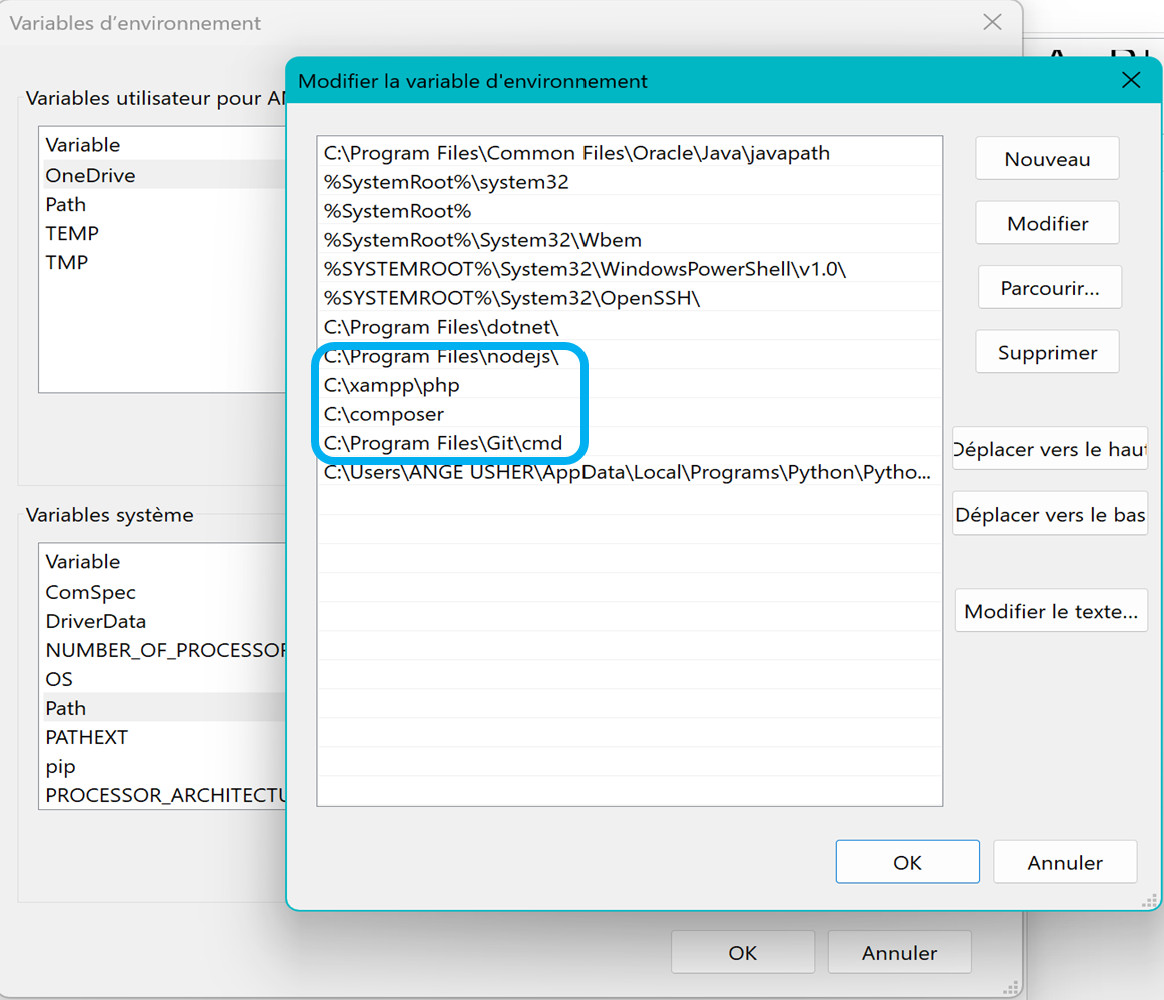
\includegraphics[width=0.58\textwidth]{./img/path.png} 
            \caption{vue sur le path}
            \label{fig:vue sur le path}
        \end{figure}   

\subsubsection{Générer la clé d'application}
Ouvrez le dossier laravel10 avec VS Code et lancez un terminal. Pour générer une nouvelle clé d'application, exécutez la commande suivante:
\medskip
        \begin{lstlisting}
php artisan key:generate
        \end{lstlisting}
\bigskip
    
\subsubsection{Configurer XAMPP et les serveurs Apache et MySQL}
Ouvrez Xampp et lancez les serveurs Apache et MySQL.
        \begin{figure}[h!] 
            \centering 
            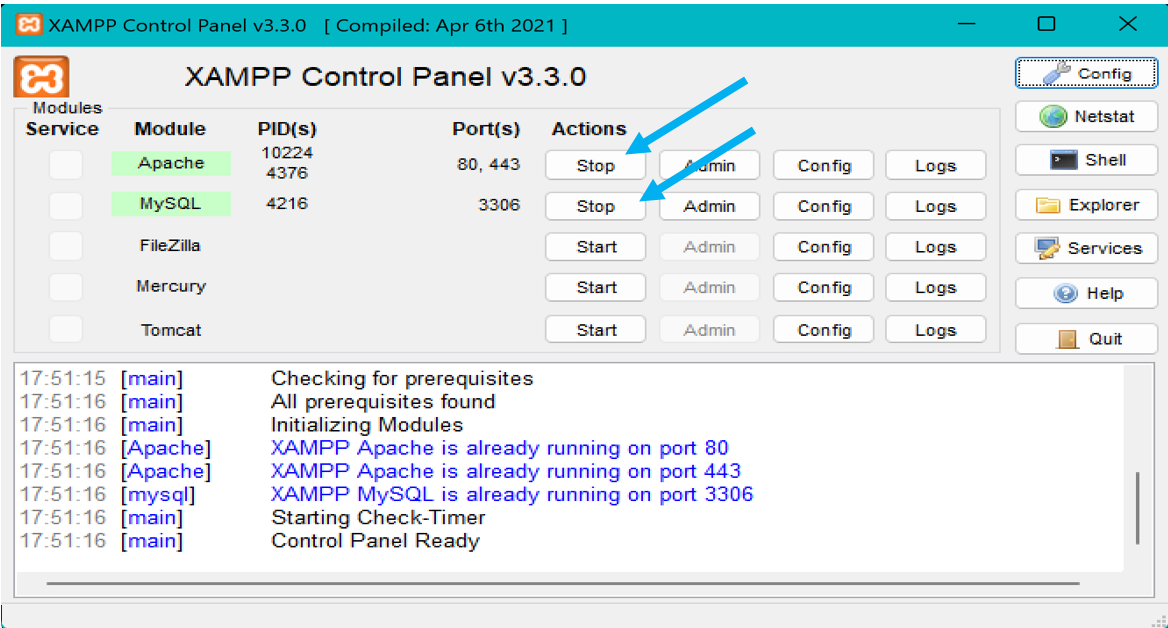
\includegraphics[width=0.7\textwidth]{./img/xampp.png}
            \caption{lancement des serveurs}
            \label{fig:lancement des serveurs} 
        \end{figure}
\bigskip

\subsubsection{Créer la base de données sur MySQL}
Ouvrez Xampp et cliquez sur le bouton Admin situé après le bouton Start pour le serveur MYSQL. La page web PhpMyAdmin  chargera et vous n'aurez qu'à créer une base de données pour l'application.   
\bigskip 

\subsubsection{Remplacer le fichier elasticsearch.yml selon votre OS} 
Il faut procéder comme suit:
\smallskip
\newline
- Téléchargez Elasticsearch (depuis le site officiel) et procédez à l'extraction de l'archive dans le répertoire de votre choix (si vous ne l'aviez pas fait précédemment).
\newline
- Copiez le fichier elasticsearch.yml fourni dans le dépôt à l'emplacement de configuration d'Elasticsearch : 
\medskip
        \begin{itemize}
            \item  Avec Windows :
            \begin{lstlisting}
copy config\elasticsearch\elasticsearch.yml C:\chemin\vers\elasticsearch\config\
            \end{lstlisting}
\newpage
            \item Avec Linux :
            \begin{lstlisting}
/bin/cp config/elasticsearch/elasticsearch.yml /chemin/vers/elasticsearch/config/
            \end{lstlisting}
        \end{itemize}
\bigskip

- Configurez le fichier elasticsearch.yml :
\medskip
    \begin{lstlisting}
SCOUT_DRIVER=Matchish\ScoutElasticSearch\Engines\ElasticSearchEngine
ELASTICSEARCH_HOST=http://localhost:9200
ELASTICSEARCH_USER=elastic
ELASTICSEARCH_PASSWORD=changeme
    \end{lstlisting}

\subsubsection{Lancer Elasticsearch}
Ouvrez un nouveau terminal et positionnez-vous sur le répertoire d'installation d'Elasticsearch. Procédez ensuite au lancement. Pour ce faire, exécutez les commandes:
        \begin{lstlisting}
#  pour Windows, tapez:
cd chemin_vers_elasticsearch\bin
elasticsearch.bat
# pour Linux, tapez:
cd cd chemin_vers_elasticsearch\bin
elasticsearch
        \end{lstlisting}
\bigskip
\bigskip
Votre terminal affichera un résultat similaire à :
    \begin{figure}[h] 
        \centering 
        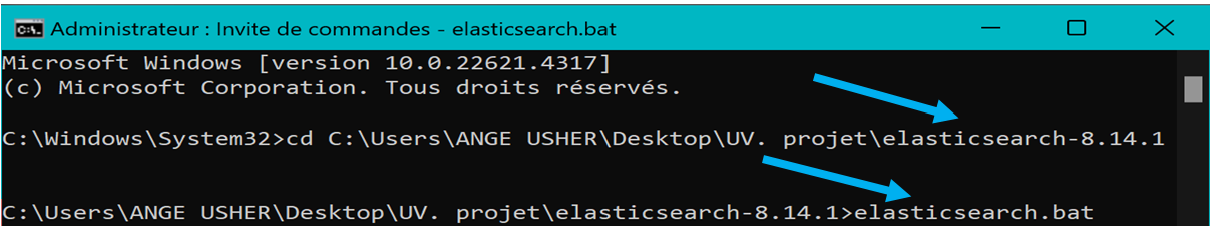
\includegraphics[width=0.8\textwidth]{./img/elastix.png} 
        \caption{vue sur le terminal d'Elasticsearch}
        \label{fig:vue sur le terminal d'Elasticsearch}
    \end{figure}
\bigskip

\subsubsection{Lancer le backend avec Laravel}
Dans un nouveau terminal, exécutez les commandes suivantes pour vous positionner sur le répertoire du dossier backend(dossier Laravel 10 plus précisémment) et procéder au lancement:
\smallskip
        \begin{lstlisting}
cd chemin\vers\backend
php artisan migrate:refresh --seed
php artisan serve
        \end{lstlisting}
\bigskip

\subsubsection{Lancer le frontend avec Angular}   
Dans un nouveau terminal, exécutez les commandes suivantes pour vous positionner sur le répertoire du dossier front-end et procéder au lancement:
\smallskip
        \begin{lstlisting}
cd chemin\vers\frontend
ng serve
        \end{lstlisting}
\bigskip
\medskip
L'application va commencer à builder et affichera à la fin de l'opération :
    \begin{figure}[h] 
        \centering 
        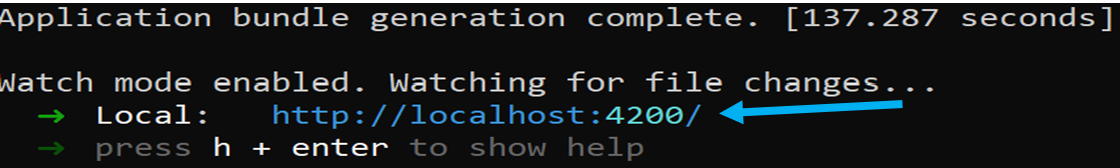
\includegraphics[width=0.8\textwidth]{./img/angular.png} 
        \caption{vue sur le terminal d'Angular}
        \label{fig:vue sur le terminal d'Angular}
    \end{figure}
\bigskip    

Enfin, copiez l'url fournie dans votre navigateur :" http://localhost:4200/ "

\vspace{0.7cm}
La page suivante s'affichera:
\smallskip
    \begin{figure}[h]
        \centering
        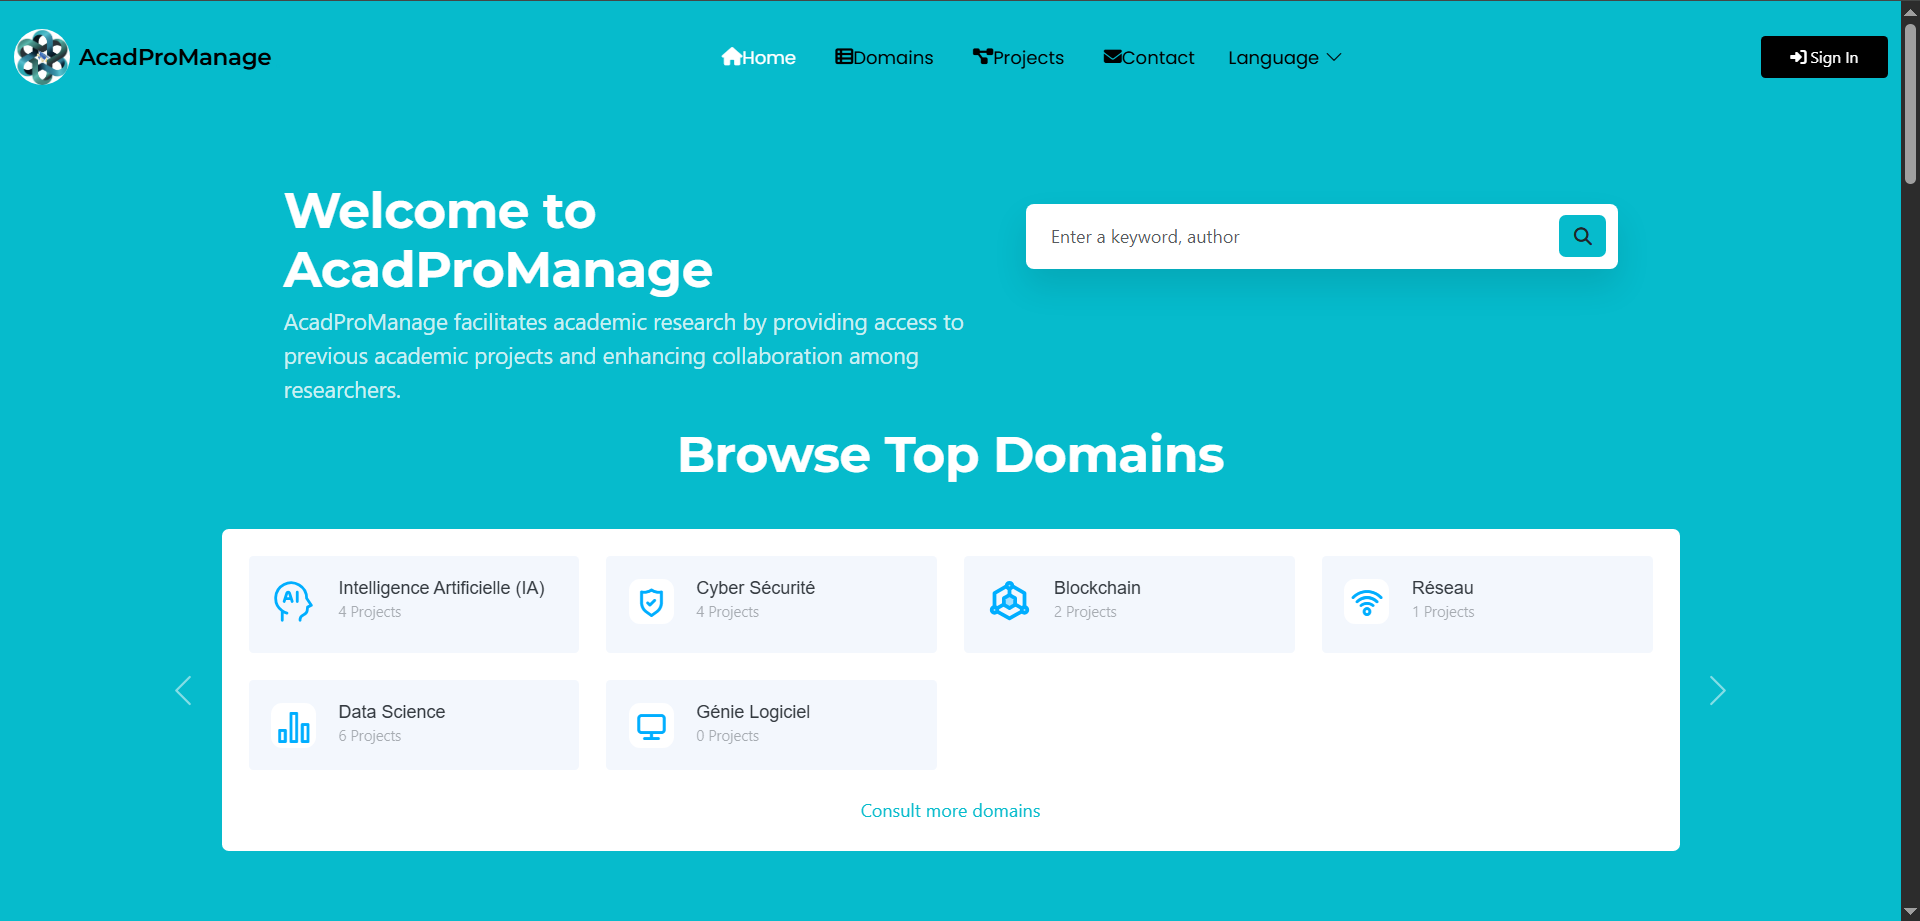
\includegraphics[width=0.8\textwidth]{./img/accueil.png}
        \caption{vue sur l'accueil}
        \label{fig:vue sur l'accueil}
    \end{figure}

\vspace{0.7cm}

{\fontsize{14}{16}\section*{Problèmes courants }}
\addcontentsline{toc}{section}{Problèmes courants }
%{\fontsize{14}{16}\textbf{\textit{Problèmes courants :}}}
Voici les problèmes majeurs que nous avons rencontrés et les solutions que nous avons adoptées pour y remédier:
\medskip
\begin{itemize}
    \item \textbf{Erreur de connexion à la base de données :} Vérifiez les identifiants dans `.env`,rassurez-vous que les serveurs Apache et MySQL sont actifs.
    \item \textbf{Problème avec Elasticsearch :} Assurez-vous qu’il est bien démarré et que le numéro de port est correct.
\end{itemize}

\newpage
% Conclusion
{\fontsize{14}{16}\section*{Conclusion}}
\addcontentsline{toc}{section}{Conclusion}
Au vu des difficultés liées à la prise en main des applications, nous avons été appelés à mettre sur pied ce petit manuel d'assistance au déploiement de notre application. Nous y avons donc mentionné les points clés à prendre en compte pour ledit déploiement, ainsi que les difficultés que nous avons rencontrées durant cette phase. En suivant les étapes décrites, les développeurs pourront exploiter pleinement l'application tout en s'assurant de sa 
pérennité et de son efficacité. Nous espérons grandement que ce manuel vous apportera le soutient nécessaire pour y arriver sereinement. Et, dans des temps futurs, nous comptons sur l'ingéniosité des développeurs et administrateurs pour y apporter des ajustements encore plus intéressants!
\end{document}